\chapter{Introduction}
\section{Common equations}

\textbf{Stefan Boltzmann Equation}: related luminosity to temperature.
\begin{equation}
    L = 4 \pi R^2 \sigma_{SB} T^4
\end{equation}
where $\sigma_{SB}$ = 5.67 $\times$ 10$^{-8}$ W m$^{-1}$ K$^{-4}$.
The sun's effective temperature is 5780 K.

\section{Stellar spectra}
\begin{enumerate}
    \item The hottest stars are the bluest.
    \item Cool stars have absorption lines of neutral atoms or molecules and are usually redder.
    \item Balmer lines are relatively weak in O-type stars because hydrogen is almost fully ionized.
    \item A-type stars have the strongest Balmer lines because they are cool enough for hydrogen in the atmosphere to be largely neutral.
    \item \textit{\textbf{Are M-stars rich in Titanium?}} M-stars, cooler than 4000 K, show strong absorption bands of Titanium and Vanadium Oxide. It is NOT because M-type stars are rich in Titanium but because these molecules absorb red light very efficiently, and the atmosphere is cool enough for the molecules not to break apart. 
    \item Bands of TiO and VO are much weaker in L-type stars than M-type stars because most of the titanium and vanadium have condensed onto dust grains.
    
\end{enumerate}

\begin{figure}
    \centering
    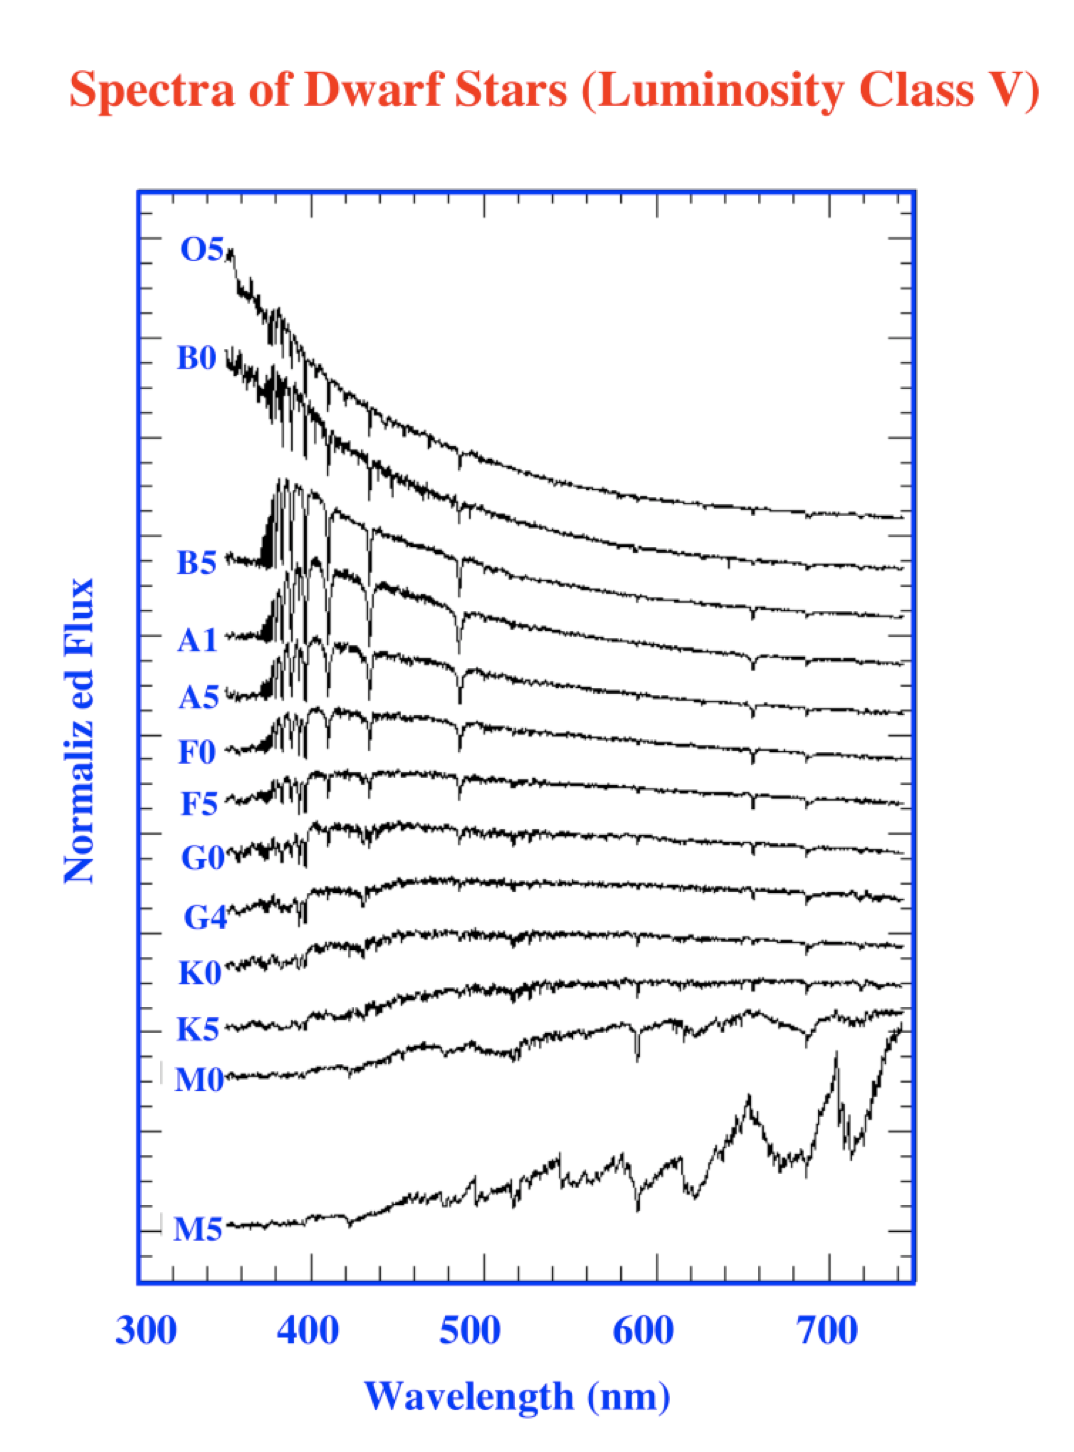
\includegraphics[scale=0.75]{Notes_Images/stellar_spectra.png}
    \caption{Stellar spectra from hottest to coldest. Notice how Balmer lines begin appearing only in A-type stars.}
    \label{fig:enter-label}
\end{figure}
\newpage
\begin{figure}
    \centering
    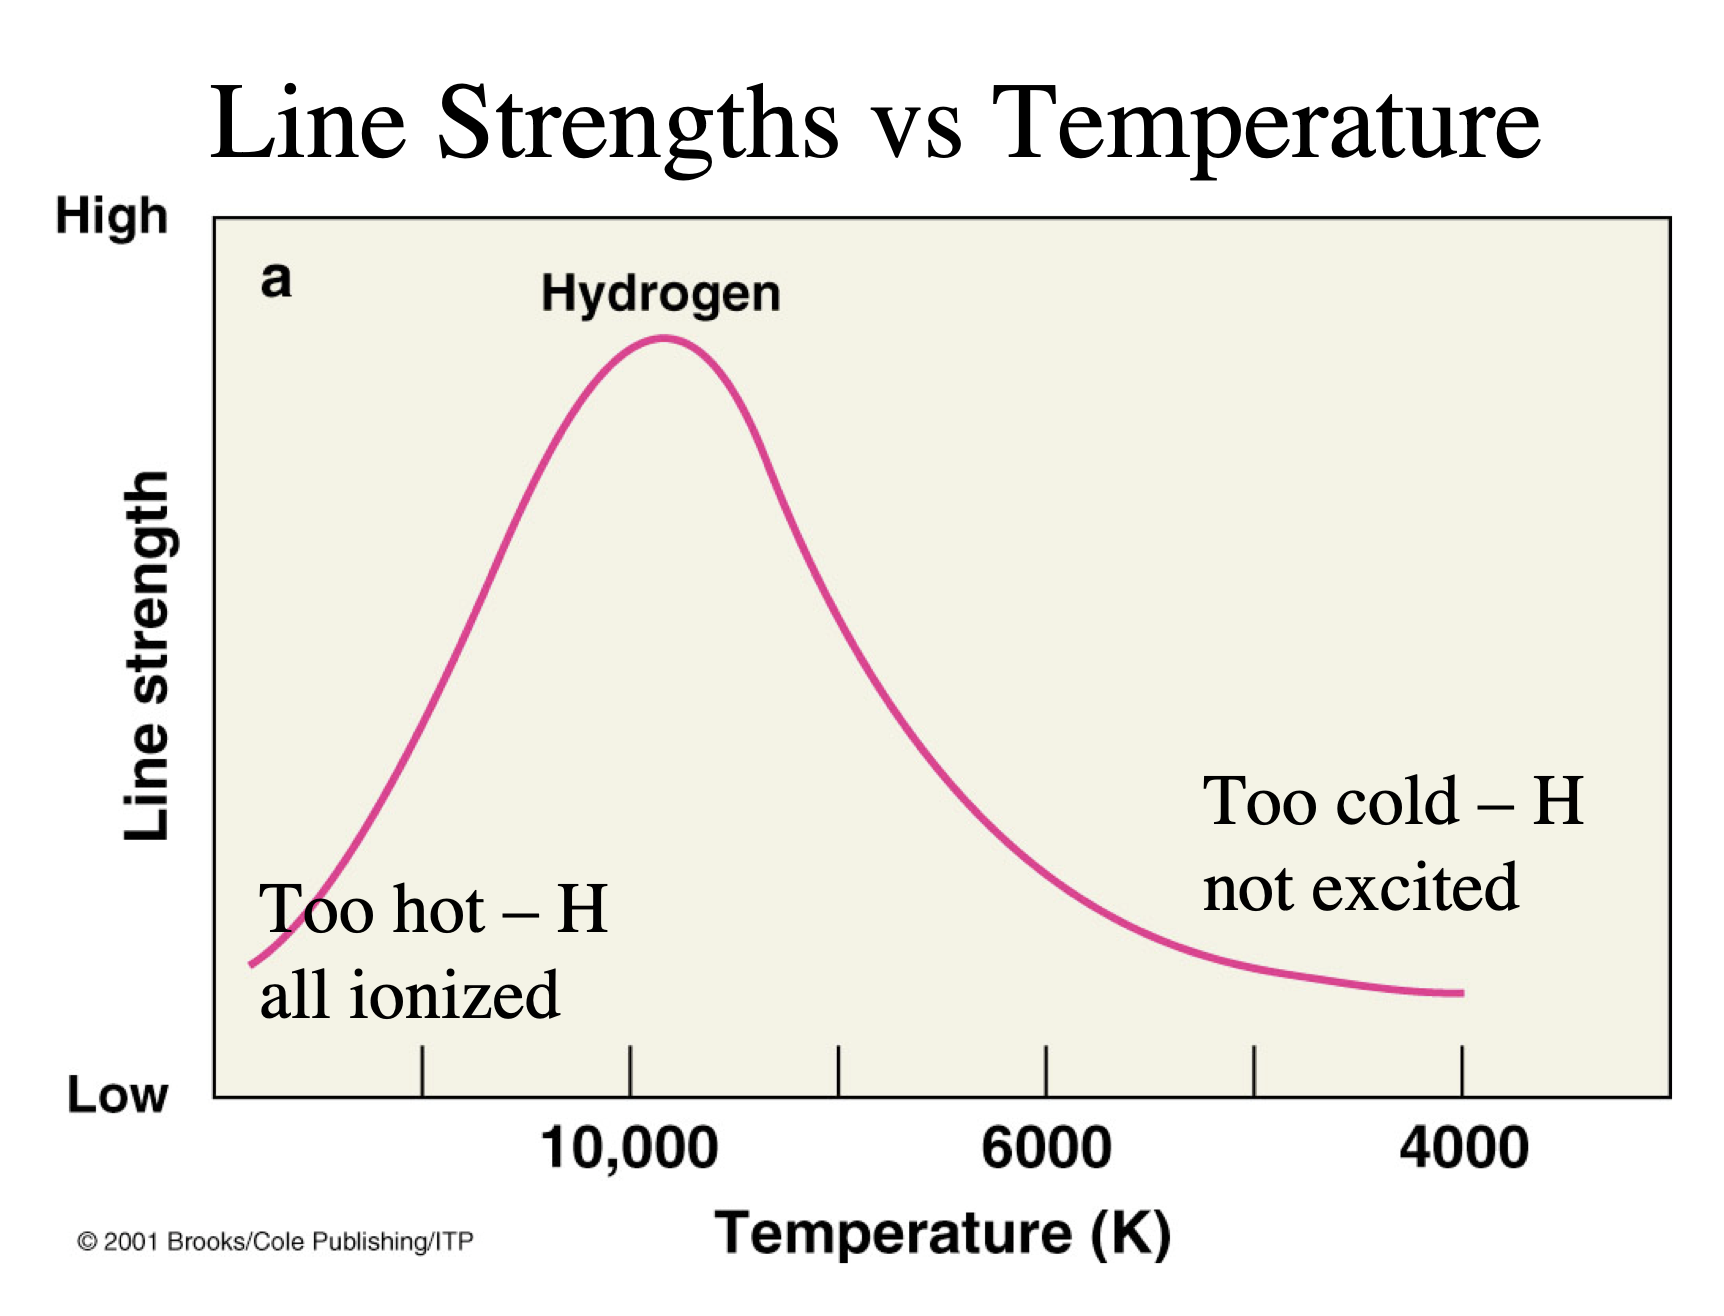
\includegraphics[scale=0.4]{Notes_Images/ionisation2.png}
    \caption{Caption}
    \label{fig:enter-label}
\end{figure}
\begin{figure}
    \centering
    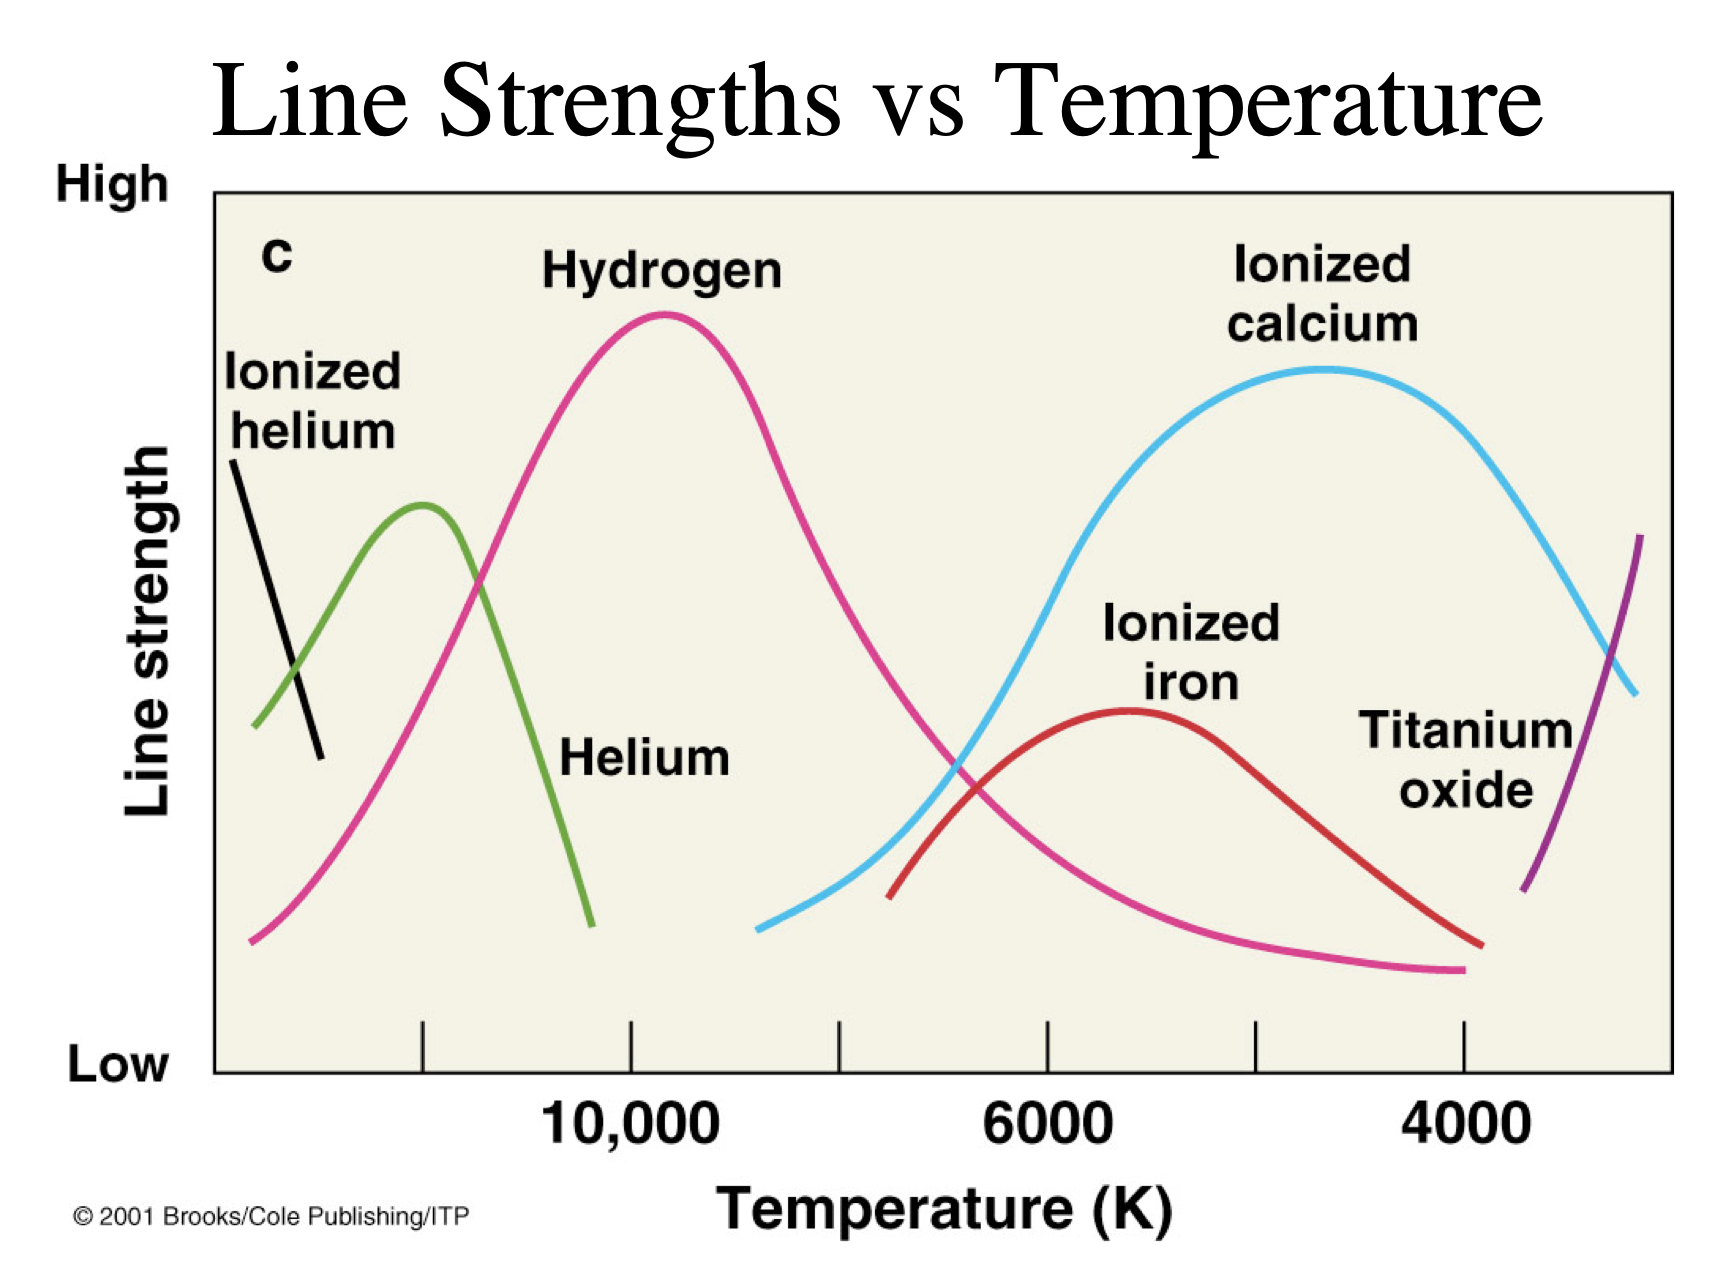
\includegraphics[scale=0.4]{Notes_Images/ionisation1.png}
    \caption{Caption}
    \label{fig:enter-label}
\end{figure}
\newpage